%FRACTIONS AS PARTS OF A WHOLE - WORKSHEET 0 (IN-CLASS INSTRUCTION)
\documentclass[12pt, letterpaper, fleqn]{article}

% ----------------------------------------------------------
% PACKAGES
% ----------------------------------------------------------
\usepackage{graphicx}
\usepackage{xcolor}
\usepackage[most]{tcolorbox}
\usepackage{amsmath, amssymb}
\usepackage{fancyhdr}
\usepackage[utf8]{inputenc}
\usepackage[T1]{fontenc}
\usepackage{enumitem}
\usepackage{geometry}
\usepackage{tikz}
\usepackage{needspace}
\usepackage{multicol}

\usetikzlibrary{arrows.meta, calc, shapes.geometric}

% ----------------------------------------------------------
% PAGE SETUP
% ----------------------------------------------------------
\usepackage{times}
\geometry{letterpaper, top=1.25in, bottom=1.25in, marginpar=0.5in}

% ----------------------------------------------------------
% HEADER / FOOTER
% ----------------------------------------------------------
\newcommand{\logowidth}{3cm}
\setlength{\headheight}{20pt}
\setlength{\footskip}{40pt}

\pagestyle{fancy}
\fancyhf{}
\fancyhead[C]{\small\bfseries Fractions as Parts of a Whole}
\fancyfoot[L]{\raisebox{2pt}{
\includegraphics[width=\logowidth]{../kss.png}}}
\fancyfoot[C]{\thepage}
\fancyfoot[R]{3.14.0}

\renewcommand{\footrulewidth}{0.2pt}

% ----------------------------------------------------------
% THEME COLOR
% ----------------------------------------------------------
\definecolor{customteal}{HTML}{2fbdb9}

% ----------------------------------------------------------
% HELPER MACROS
% ----------------------------------------------------------
\newcommand{\blank}{\underline{\hspace{2.2cm}}}
\newcommand{\blanklong}{\underline{\hspace{6.5cm}}}
\newcommand{\blankshorter}{\underline{\hspace{1.5cm}}}

% ----------------------------------------------------------
% DOCUMENT
% ----------------------------------------------------------
\begin{document}

\textbf{Name:} \underline{\hspace{5cm}}
\hfill
\textbf{Date:} \underline{\hspace{3cm}}\\

\begin{tcolorbox}[colback=customteal!20]
    \large\textcolor{black}{\textbf{Introduction to Fractions}}
\end{tcolorbox}

\vspace{3mm}
\noindent
A **fraction** represents equal parts of a whole object.
\[
\text{Fraction} = \frac{\text{Numerator (shaded parts)}}{\text{Denominator (total equal parts)}}
\tag{e.g., $\dfrac{2}{3}$}
\]

\begin{tcolorbox}[colback=white, colframe=black!25, boxrule=0.6pt, arc=4mm]
\textbf{Fraction Model}
\begin{center}
\begin{tikzpicture}[scale=0.8]
\draw[thick] (0,0) rectangle (4,1.2);
\foreach \x in {1,2,3} {
  \draw[thick] (\x,0) -- (\x,1.2);
}
\fill[customteal!40] (0,0) rectangle (2,1.2);
\draw[thick] (0,0) rectangle (4,1.2); % Redraw outline
\node at (2, -0.6) {2 parts out of 4 are shaded $\rightarrow \dfrac{2}{4}$};
\end{tikzpicture}
\end{center}
\end{tcolorbox}

\newpage
\begin{tcolorbox}[colback=customteal!20]
    \large\textcolor{black}{\textbf{Guided Practice}}
\end{tcolorbox}

\vspace{5mm}
\noindent
Write the fraction represented by the shaded shapes.

\vspace{8mm}
\begin{enumerate}[itemsep=3cm, leftmargin=0.6cm]
\item 
\begin{tikzpicture}[scale=0.8]
\draw[thick] (0,0) circle(1cm);
\draw[thick] (-1,0) -- (1,0);
\draw[thick] (0,-1) -- (0,1);
\fill[customteal!30] (0,0) -- (0,1) arc(90:270:1) -- cycle;
\end{tikzpicture}
\\
Fraction: \blank

\item 
\begin{tikzpicture}[scale=0.8]
\draw[thick] (0,0) rectangle (3,1);
\draw[thick] (1,0) -- (1,1);
\draw[thick] (2,0) -- (2,1);
\fill[customteal!30] (0,0) rectangle (1,1);
\end{tikzpicture}
\\
Fraction: \blank
\end{enumerate}

\end{document}
